% ======================================================================
%  Appendix A — Vector Identities and Functional Analysis  (EXPANDED)
% ======================================================================

\section{Vector calculus identities}
\label{sec:appA-vector}

\subsection{Fundamental differential identities}
\label{sec:appA-differential}

The following identities are used throughout the derivations of
Chapters~2--5.  All fields are assumed sufficiently smooth.

For any scalar field $\phi$ and vector fields $\mathbf{F}$,
$\mathbf{G}$:
\begin{align}
  \nabla\times(\nabla\phi) &= \mathbf{0}\,,
    \label{eq:appA-curl-grad}\\
  \nabla\cdot(\nabla\times\mathbf{F}) &= 0\,,
    \label{eq:appA-div-curl}\\
  \nabla\times(\nabla\times\mathbf{F})
    &= \nabla(\nabla\cdot\mathbf{F})-\nabla^2\mathbf{F}\,,
    \label{eq:appA-curl-curl}\\
  \nabla\cdot(\phi\mathbf{F})
    &= \phi\,\nabla\cdot\mathbf{F}
    +\mathbf{F}\cdot\nabla\phi\,,
    \label{eq:appA-div-product}\\
  \nabla\times(\phi\mathbf{F})
    &= \phi\,\nabla\times\mathbf{F}
    +(\nabla\phi)\times\mathbf{F}\,.
    \label{eq:appA-curl-product}
\end{align}
The double-curl identity \eqref{eq:appA-curl-curl} is especially
important: it converts the Maxwell wave equation into a Helmholtz
equation for a divergence-free field.

For products of two vector fields:
\begin{align}
  \nabla\cdot(\mathbf{F}\times\mathbf{G})
    &= \mathbf{G}\cdot(\nabla\times\mathbf{F})
    -\mathbf{F}\cdot(\nabla\times\mathbf{G})\,,
    \label{eq:appA-div-cross}\\
  \nabla(\mathbf{F}\cdot\mathbf{G})
    &= (\mathbf{F}\cdot\nabla)\mathbf{G}
    +(\mathbf{G}\cdot\nabla)\mathbf{F}
    +\mathbf{F}\times(\nabla\times\mathbf{G})
    +\mathbf{G}\times(\nabla\times\mathbf{F})\,.
    \label{eq:appA-grad-dot}
\end{align}

\subsection{Integral theorems}
\label{sec:appA-integral}

The divergence (Gauss) theorem:
\begin{equation}\label{eq:appA-gauss}
  \int_V\nabla\cdot\mathbf{F}\,\dd^3r
  = \oint_{\partial V}\mathbf{F}\cdot\hat{n}\,\dd S\,.
\end{equation}
The curl (Stokes) theorem:
\begin{equation}\label{eq:appA-stokes}
  \int_S(\nabla\times\mathbf{F})\cdot\hat{n}\,\dd S
  = \oint_{\partial S}\mathbf{F}\cdot\dd\boldsymbol{\ell}\,.
\end{equation}
These are used in the Poynting-theorem derivation
(\secref{sec:ch2-poynting}) and in the self-adjointness proof for
the Maxwell curl operator (\secref{sec:ch3-self-adjoint})
\cite{press2026photonic}.

\subsection{The Levi-Civita symbol and cross products}
\label{sec:appA-levi-civita}

The Levi-Civita symbol $\epsilon_{ijk}$ is defined by $\epsilon_{123}=1$
and antisymmetry under transposition of any two indices.  Cross products
and curls are expressed as
\begin{equation}\label{eq:appA-cross}
  (\mathbf{A}\times\mathbf{B})_i
  = \sum_{jk}\epsilon_{ijk}A_j B_k\,,
  \qquad
  (\nabla\times\mathbf{F})_i
  = \sum_{jk}\epsilon_{ijk}\partial_j F_k\,.
\end{equation}
The contracted product identity is
\begin{equation}\label{eq:appA-eps-contract}
  \sum_k\epsilon_{ijk}\epsilon_{klm}
  = \delta_{il}\delta_{jm}-\delta_{im}\delta_{jl}\,,
\end{equation}
from which many vector identities follow algebraically.

\section{The Maxwell integration-by-parts lemma}
\label{sec:appA-ibp}

\subsection{Statement}
\label{sec:appA-ibp-statement}

The central analytic tool in Chapters~2--3 is the integration-by-parts
identity for the six-component Maxwell curl operator $\Maxop$.

\begin{proposition}[Maxwell integration by parts]
\label{prop:appA-ibp}
For six-component fields $\emfield_1=(\Efield_1,\Hfield_1)^T$ and
$\emfield_2=(\Efield_2,\Hfield_2)^T$ on a domain $\Omega$ with
boundary $\partial\Omega$:
\begin{equation}\label{eq:appA-ibp}
  \int_\Omega\emfield_1^\dagger\,\Maxop\,\emfield_2\,\dd^3r
  - \int_\Omega(\Maxop\,\emfield_1)^\dagger\,\emfield_2\,\dd^3r
  = \oint_{\partial\Omega}\bigl[
    (\hat{n}\times\Efield_1^*)^T\Hfield_2
    - (\hat{n}\times\Hfield_1^*)^T\Efield_2
  \bigr]\,\dd S\,.
\end{equation}
\end{proposition}

The identity is more than a vector-calculus convenience.  It says that
self-adjointness of Maxwell's curl block is decided at the boundary,
not in the bulk algebra alone.  Figure~\ref{fig:appA-ibp-boundary}
shows this logic: the volume commutator of the curl operator is
converted into tangential electric and magnetic traces on
$\partial\Omega$.  Periodic boundary conditions, perfectly conducting
walls, or decay at infinity remove this boundary pairing; an interface
problem keeps it, and that surviving term is the analytic shadow of an
edge channel.

\begin{figure}[t]
  \centering
  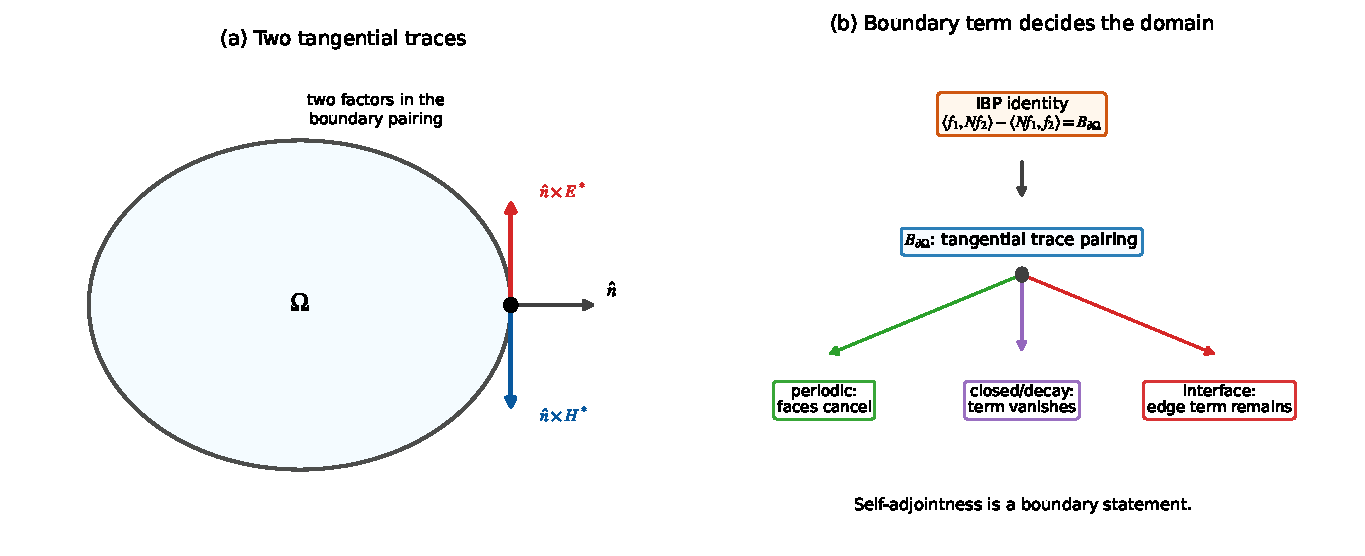
\includegraphics[width=0.94\textwidth]{figures/fig_appA_ibp_boundary.pdf}
  \caption{The Maxwell integration-by-parts identity as a boundary
  statement.  The difference between the two curl-block matrix elements
  is a surface pairing of tangential field traces.  When opposite
  faces cancel, fields decay, or boundary conditions set the trace
  pairing to zero, the Maxwell curl block becomes symmetric on the
  chosen domain.  At an interface the same boundary term is the place
  where edge-mode physics enters the operator proof.}
  \label{fig:appA-ibp-boundary}
\end{figure}


\subsection{Derivation}
\label{sec:appA-ibp-proof}

We start from the divergence identity \eqref{eq:appA-div-cross}:
\begin{equation}
  \nabla\cdot(\Efield_1^*\times\Hfield_2)
  = \Hfield_2\cdot(\nabla\times\Efield_1^*)
  - \Efield_1^*\cdot(\nabla\times\Hfield_2)\,.
\end{equation}
Similarly:
\begin{equation}
  \nabla\cdot(\Hfield_1^*\times\Efield_2)
  = \Efield_2\cdot(\nabla\times\Hfield_1^*)
  - \Hfield_1^*\cdot(\nabla\times\Efield_2)\,.
\end{equation}
Adding these two expressions and rearranging in terms of the
six-component operator $\Maxop$ gives \eqref{eq:appA-ibp}.  Applying
the divergence theorem converts the divergence terms into the surface
integral over $\partial\Omega$.

When the boundary term vanishes (e.g.\ for periodic boundary conditions,
perfectly conducting walls, or fields that decay at infinity), the
curl operator $\Maxop$ is formally self-adjoint under the bare $L^2$
inner product.  The physical self-adjointness under the energy inner
product $\langle\cdot|\Mmat|\cdot\rangle$ follows from
$\Maxop^\dagger=\Maxop$ combined with $\Mmat=\Mmat^\dagger$
(lossless medium).

\section{Spectral theory of self-adjoint operators}
\label{sec:appA-spectral}

\subsection{Finite-dimensional review}
\label{sec:appA-finite}

For a finite-dimensional Hermitian matrix $H=H^\dagger$ acting on \cite{raman2010photonic}
$\mathbb{C}^N$, the spectral theorem guarantees real eigenvalues
$\lambda_1\leq\cdots\leq\lambda_N$, a complete orthonormal basis of
eigenvectors $|v_n\rangle$, and the resolution of the identity:
\begin{equation}\label{eq:appA-spectral-finite}
  H = \sum_{n=1}^N\lambda_n\,|v_n\rangle\langle v_n|\,,
  \qquad
  \mathbf{I} = \sum_{n=1}^N|v_n\rangle\langle v_n|\,.
\end{equation}

\subsection{Extension to the Maxwell operator}
\label{sec:appA-maxwell-spectral}

The Maxwell eigenvalue problem
$\Maxop\emfield=\omega\Mmat\emfield$ on a bounded or periodic
domain, with appropriate boundary conditions, is a generalised
eigenvalue problem with a positive-definite ``weight'' $\Mmat$.  The
key spectral properties are:

All eigenfrequencies $\omega_n$ are real, because the operator
$\Mmat^{-1}\Maxop$ is self-adjoint with respect to the
$\Mmat$-weighted inner product.

The eigenmodes $\emfield_n$ are orthogonal under the energy inner
product: $\emip{\emfield_m}{\emfield_n}=\delta_{mn}$ after
normalisation.

The eigenmodes form a complete set: any sufficiently smooth field
satisfying the boundary conditions can be expanded in the eigenmode
basis.

For a periodic medium (photonic crystal), the eigenvalue problem
decomposes into a family of problems parametrised by the Bloch
wavevector $\kvec$, each of which has a discrete spectrum
$\{\omega_{n\kvec}\}_{n=1}^\infty$.  As $\kvec$ varies over the
Brillouin zone, these eigenvalues trace the photonic band structure.

\subsection{The min-max principle}
\label{sec:appA-minmax}

The min-max (Courant--Fischer) characterisation of eigenvalues
provides variational bounds:
\begin{equation}\label{eq:appA-minmax}
  \omega_n^2 = \min_{\dim V=n}\max_{\emfield\in V\backslash\{0\}}
  \frac{\langle\emfield|\Maxop^2|\emfield\rangle}
  {\emip{\emfield}{\emfield}}\,.
\end{equation}
This is the electromagnetic analog of the Rayleigh--Ritz variational
principle in quantum mechanics \cite{nittis2020equivalence}.  It is used in perturbation theory
to bound the frequency shifts caused by material changes \cite{atala2013direct}.

\section{Perturbation theory for the Maxwell eigenproblem}
\label{sec:appA-perturbation}

\subsection{Non-degenerate perturbation theory}
\label{sec:appA-nondegenerate}

Consider a perturbation $\Mmat\to\Mmat+\delta\Mmat$ of the material
matrix.  The first-order frequency shift of a non-degenerate mode
$\emfield_n$ is
\begin{equation}\label{eq:appA-first-order}
  \delta\omega_n
  = -\frac{\omega_n}{2}\,
  \frac{\langle\emfield_n|\delta\Mmat|\emfield_n\rangle}
  {\emip{\emfield_n}{\emfield_n}}\,.
\end{equation}
This is the electromagnetic Hellmann--Feynman theorem; it appears in
Equation~\eqref{eq:ch4-hellmann-feynman} and is used extensively in Chapters~7
and~11.

\subsection{Degenerate perturbation theory}
\label{sec:appA-degenerate}

When two or more modes are degenerate at $\omega_0$, the first-order
correction is found by diagonalising the perturbation within the
degenerate subspace.  Let $\{|\emfield_\alpha\rangle\}_{\alpha=1}^p$
be the degenerate modes.  The first-order frequency splittings are the
eigenvalues of the $p\times p$ matrix:
\begin{equation}\label{eq:appA-degenerate}
  V_{\alpha\beta}
  = -\frac{\omega_0}{2}\,
  \frac{\langle\emfield_\alpha|\delta\Mmat|\emfield_\beta\rangle}
  {\emip{\emfield_\alpha}{\emfield_\alpha}}\,.
\end{equation}
This is the key formula for deriving the effective Dirac Hamiltonian
at high-symmetry points (Chapter~6) and the mass terms from
time-reversal or inversion breaking (Chapters~7, 11, 12).

\section{Function spaces and boundary conditions}
\label{sec:appA-function-spaces}

\subsection{The relevant Sobolev spaces} \cite{initio2026pdf}
\label{sec:appA-sobolev}

The natural function space for the Maxwell eigenvalue problem is the
space of square-integrable vector fields with square-integrable curl:
\begin{equation}\label{eq:appA-hcurl}
  H(\mathrm{curl},\Omega)
  = \bigl\{\mathbf{F}\in L^2(\Omega)^3
  \;\big|\;\nabla\times\mathbf{F}\in L^2(\Omega)^3\bigr\}\,.
\end{equation}
This is the electromagnetic analog of the Sobolev space $H^1$.  The
boundary conditions (perfect conductor, periodic, or radiation) are
imposed by restricting to appropriate subspaces.

For periodic media (photonic crystals), the relevant space is the
Bloch-periodic version:
\begin{equation}\label{eq:appA-bloch-space}
  H_\kvec(\mathrm{curl},\Omega_{\mathrm{cell}})
  = \bigl\{\mathbf{F}\in H(\mathrm{curl},\Omega_{\mathrm{cell}})
  \;\big|\;
  \mathbf{F}(\rvec+\avec)=\ee^{\ii\kvec\cdot\avec}\mathbf{F}(\rvec)
  \;\forall\;\avec\in\Lambda\bigr\}\,,
\end{equation}
where $\Lambda$ is the Bravais lattice.

\subsection{Completeness and regularity}
\label{sec:appA-completeness}

For a lossless medium with positive-definite $\Mmat$, the Maxwell
eigenproblem on a bounded domain (or on a unit cell with Bloch boundary
conditions) has a discrete spectrum accumulating at infinity.  The
eigenmodes form a complete orthonormal basis in the $\Mmat$-weighted
$L^2$ space.

For smooth material parameters ($\Mmat\in C^\infty$), the eigenmodes
are themselves smooth inside the domain.  At material interfaces where
$\Mmat$ has jump discontinuities, the tangential components of
$\Efield$ and $\Hfield$ remain continuous, but normal components may
have jumps proportional to the contrast.

\section{Useful matrix identities}
\label{sec:appA-matrix}

For $2\times 2$ matrices expressed in terms of Pauli matrices,
$H=d_0\mathbf{I}+\mathbf{d}\cdot\boldsymbol{\sigma}$:
\begin{align}
  \det(H) &= d_0^2 - |\mathbf{d}|^2\,,\\
  \Tr(H) &= 2d_0\,,\\
  H^{-1} &= \frac{d_0\mathbf{I}-\mathbf{d}\cdot\boldsymbol{\sigma}}
  {d_0^2-|\mathbf{d}|^2}\,,\\
  \ee^{\ii\theta\,\hat{n}\cdot\boldsymbol{\sigma}}
  &= \cos\theta\,\mathbf{I}+\ii\sin\theta\,
  \hat{n}\cdot\boldsymbol{\sigma}\,.
\end{align}
The Pauli-matrix trace identities are:
\begin{align}
  \Tr(\sigma_a) &= 0\,,\\
  \Tr(\sigma_a\sigma_b) &= 2\delta_{ab}\,,\\
  \Tr(\sigma_a\sigma_b\sigma_c) &= 2\ii\epsilon_{abc}\,.
\end{align}
These identities are used extensively in the effective-Hamiltonian
derivations of Chapters~6--8, 11--12, and 15.

\section{The Baker--Campbell--Hausdorff formula}
\label{sec:appA-bch}

For operators $A$ and $B$:
\begin{equation}\label{eq:appA-bch}
  \ee^A\ee^B = \exp\Bigl(A+B+\frac{1}{2}[A,B]
  +\frac{1}{12}\bigl([A,[A,B]]+[B,[B,A]]\bigr)+\cdots\Bigr)\,.
\end{equation}
This is used in the derivation of the Wilson loop
(\secref{sec:ch5-wilson}) and in the analysis of Floquet evolution
operators (Chapter~\ref{ch:floquet}).

\section{The electromagnetic Green's function}
\label{sec:appA-green}

\subsection{Definition and properties}
\label{sec:appA-green-def}

The Green's function (resolvent kernel) of the Maxwell operator is
defined by
\begin{equation}\label{eq:appA-green-def}
  \bigl(\Maxop - \omega\,\Mmat\bigr)\,
  \mathbf{G}(\rvec,\rvec';\omega)
  = \delta^{(3)}(\rvec-\rvec')\,\mathbf{I}_6\,,
\end{equation}
where $\mathbf{I}_6$ is the $6\times 6$ identity.  Formally, the
Green's function is the kernel of the resolvent operator
$R(\omega)=(\Maxop-\omega\Mmat)^{-1}$:
\begin{equation}\label{eq:appA-resolvent}
  R(\omega) = \sum_n
  \frac{|\emfield_n\rangle\langle\emfield_n|\Mmat}
  {\omega_n-\omega}\,,
\end{equation}
where the sum runs over the complete set of eigenmodes.  The poles of
$R(\omega)$ are the eigenfrequencies $\omega_n$, and the residue at
each pole projects onto the corresponding eigenmode.

\subsection{Spectral representation in periodic media}
\label{sec:appA-green-periodic}

For a photonic crystal, the Green's function decomposes over Bloch
wavevectors:
\begin{equation}\label{eq:appA-green-bloch}
  \mathbf{G}(\rvec,\rvec';\omega)
  = \sum_n\int_{\mathrm{BZ}}\frac{\dd^d k}{(2\pi)^d}
  \frac{\emfield_{n\kvec}(\rvec)\,
  \emfield_{n\kvec}^\dagger(\rvec')\,\Mmat}
  {\omega_{n\kvec}-\omega}\,.
\end{equation}
The imaginary part $\imag\,\Tr\,\mathbf{G}(\rvec,\rvec;\omega+\ii 0^+)$
gives the local density of states
\cite{ozawa2018topological}:
\begin{equation}\label{eq:appA-ldos}
  \rho(\rvec,\omega)
  = -\frac{1}{\pi}\imag\,\Tr\bigl[\Mmat\,
  \mathbf{G}(\rvec,\rvec;\omega+\ii 0^+)\bigr]\,.
\end{equation}
This relation connects the spectral properties of the Maxwell operator
(through the Green's function poles) to the experimentally observable
local density of states.

\subsection{Gap Chern number from the Green's function}
\label{sec:appA-green-chern}

The Chern number can be expressed directly in terms of the Green's
function, without requiring explicit knowledge of the eigenmodes.
For a frequency $\omega$ lying in a spectral gap, the gap Chern number
is \cite{silveirinha2016bulk}
\begin{equation}\label{eq:appA-chern-green}
  \Chern_{\mathrm{gap}}(\omega)
  = \frac{\epsilon_{ab}}{4\pi\ii}\int_{\mathrm{BZ}}
  \Tr\bigl[
    G\,\partial_{k_a}G^{-1}\,G\,\partial_{k_b}G^{-1}
  \bigr]\,\dd^2 k\,,
\end{equation}
where $G\equiv\mathbf{G}(\kvec;\omega)$ is the $\kvec$-dependent
Green's function evaluated at the gap frequency.  This formula is
especially useful for non-Hermitian and continuum systems where the
eigenmode basis may not be well defined \cite{gangaraj2016berry}.

\section{Tensor product structure of the six-component space}
\label{sec:appA-tensor}

The six-component Maxwell field $\emfield=(\Efield,\Hfield)^T$ lives
in the direct sum $\mathcal{H}=\mathcal{H}_E\oplus\mathcal{H}_H$,
where $\mathcal{H}_E$ and $\mathcal{H}_H$ are the spaces of
square-integrable 3-component electric and magnetic fields
respectively.  The material matrix $\Mmat$ and the curl operator
$\Maxop$ have specific block structures in this decomposition:
\begin{equation}\label{eq:appA-block-M}
  \Mmat = \begin{pmatrix}
    \varepsilon_0\epst & 0 \\ 0 & \mu_0\mut
  \end{pmatrix},
  \qquad
  \Maxop = \begin{pmatrix}
    0 & \nabla\times \\
    -\nabla\times & 0
  \end{pmatrix},
\end{equation}
in the absence of bianisotropy ($\xit=\zetat=0$).  The off-diagonal
structure of $\Maxop$ couples the electric and magnetic sectors, while
the block-diagonal structure of $\Mmat$ separates them.  This
``chiral'' structure is the origin of many symmetry properties:
for example, $\Maxop$ anticommutes with the matrix
$\sigma_3=\mathrm{diag}(\mathbf{I}_3,-\mathbf{I}_3)$, so that
eigenfrequencies come in $\pm\omega$ pairs for lossless media.

When bianisotropic coupling $\xit\neq 0$ is present (as in the
Khanikaev metamaterial of Chapter~\ref{ch:reciprocal-designs}), the
material matrix acquires off-diagonal blocks, and the direct-sum
decomposition breaks down.  The pseudospin topology of
Chapter~\ref{ch:reciprocal-designs} can be understood as a controlled
restoration of this decomposition through the bianisotropic coupling.

\section{Proof of the curl-curl identity}
\label{sec:appA-curl-curl-proof}

The double-curl identity $\nabla\times(\nabla\times\mathbf{F})
=\nabla(\nabla\cdot\mathbf{F})-\nabla^2\mathbf{F}$ is fundamental to
the reduction of the Maxwell wave equation to the Helmholtz equation.
We give a component-wise proof using the Levi-Civita symbol.

\begin{proof}
The $i$-th component of $\nabla\times(\nabla\times\mathbf{F})$ is
\begin{equation}
  [\nabla\times(\nabla\times\mathbf{F})]_i
  = \epsilon_{ijk}\partial_j(\nabla\times\mathbf{F})_k
  = \epsilon_{ijk}\epsilon_{klm}\partial_j\partial_l F_m\,.
\end{equation}
Using the contraction identity $\epsilon_{ijk}\epsilon_{klm}
=\delta_{il}\delta_{jm}-\delta_{im}\delta_{jl}$:
\begin{align}
  [\nabla\times(\nabla\times\mathbf{F})]_i
  &= (\delta_{il}\delta_{jm}-\delta_{im}\delta_{jl})
  \partial_j\partial_l F_m \notag\\
  &= \partial_j\partial_i F_j - \partial_j\partial_j F_i \notag\\
  &= \partial_i(\nabla\cdot\mathbf{F}) - \nabla^2 F_i\,.
\end{align}
This is the $i$-th component of
$\nabla(\nabla\cdot\mathbf{F})-\nabla^2\mathbf{F}$.
\end{proof}

\section{Self-adjoint extensions and boundary conditions}
\label{sec:appA-selfadjoint}

\subsection{The domain of the curl operator}
\label{sec:appA-curl-domain}

The Maxwell curl operator $\Maxop$ is formally defined on smooth,
compactly supported 6-component fields \cite{bernevig2006quantum}.  To make $\Maxop$
self-adjoint in the Hilbert space
$\mathcal{H}=L^2(\Omega;\Mmat\,\dd V)$ (with the electromagnetic
energy inner product), one must specify boundary conditions.

On a domain $\Omega$ with boundary $\partial\Omega$, the natural
boundary condition for the lossless Maxwell problem is the perfect
electric conductor (PEC) condition:
\begin{equation}\label{eq:appA-pec}
  \hat{n}\times\Efield\big|_{\partial\Omega} = 0\,,
\end{equation}
where $\hat{n}$ is the outward unit normal.  With this condition, the
integration-by-parts identity
\begin{equation}\label{eq:appA-ibp-maxwell}
  \emip{\emfield_1}{\Maxop\emfield_2}
  - \emip{\Maxop\emfield_1}{\emfield_2}
  = \oint_{\partial\Omega}
  (\Efield_1\times\Hfield_2-\Efield_2\times\Hfield_1)
  \cdot\hat{n}\,\dd S
\end{equation}
shows that the boundary term vanishes, and $\Maxop$ is symmetric
(formally self-adjoint) on the PEC domain.  A rigorous proof of
essential self-adjointness requires functional-analytic tools
(Friedrichs extension, graph norm estimates), but the key physical
insight is that the boundary conditions determine the domain of
$\Maxop$, and hence the spectrum \cite{gangaraj2016berry}.

\subsection{Boundary conditions and edge modes}
\label{sec:appA-bc-edge}

Different boundary conditions produce different self-adjoint
extensions of $\Maxop$, and hence different spectra.  The topological
edge modes discussed in Chapters~7--9 arise precisely because the
boundary changes the self-adjoint extension: the bulk operator has a
gapped spectrum, but the half-space operator (with PEC or impedance
boundary conditions) has additional eigenvalues in the gap.

The number of these in-gap eigenvalues is determined by the Chern
number of the bulk bands, through the bulk-edge correspondence.  This
is a rigorous mathematical statement: the spectral flow of the
boundary problem equals the Chern number of the bulk problem,
regardless of the specific boundary condition chosen
\cite{silveirinha2016bulk,ozawa2018topological}.

\section{Spectral theory of the Maxwell operator}
\label{sec:appA-spectral-theory}

\subsection{Essential and discrete spectrum}
\label{sec:appA-essential-discrete}

The spectrum of $\Maxop$ in a periodic medium decomposes into two
parts.  The \emph{essential spectrum} consists of the photonic bands:
continuous intervals of $\omega$ filled by propagating Bloch modes.
The \emph{discrete spectrum} consists of isolated eigenvalues
(localised defect modes or edge modes), which can appear in band gaps.

For a perfect photonic crystal (no defects, no boundaries), the
spectrum is purely essential and consists of the union of all photonic
bands.  When a boundary or defect is introduced, discrete eigenvalues
may appear in the gaps.  The topological edge modes are precisely such
discrete eigenvalues, whose existence is guaranteed by the nonzero
Chern number of the bulk bands.

\subsection{Weyl's theorem and stability of the essential spectrum}
\label{sec:appA-weyl}

Weyl's theorem states that the essential spectrum of a self-adjoint
operator is invariant under compact perturbations.  In the photonic
context, this means that local defects (finite-range changes in the
material matrix $\Mmat$) cannot change the band structure of the bulk
crystal; they can only add or remove discrete eigenvalues in the gaps.

This stability is the mathematical foundation of topological
protection: the bulk gap cannot be closed by any local perturbation,
so the edge modes that are topologically required to exist in the gap
are also protected against local perturbations
\cite{ozawa2018topological}.

\section{Bloch decomposition and direct integral}
\label{sec:appA-bloch-decomposition}

For a photonic crystal with lattice $\Lambda$, the Hilbert space
decomposes as a direct integral over the Brillouin zone:
\begin{equation}\label{eq:appA-direct-integral}
  \mathcal{H}
  = \int_{\mathrm{BZ}}^\oplus\mathcal{H}_\kvec\,\frac{\dd^d k}{(2\pi)^d}\,,
\end{equation}
where $\mathcal{H}_\kvec=L^2(\Omega_{\mathrm{cell}};\Mmat\,\dd V)$
is the Hilbert space of cell-periodic fields at fixed $\kvec$.  The
Maxwell operator decomposes correspondingly:
$\Maxop=\int_{\mathrm{BZ}}^\oplus\Maxop(\kvec)\,\dd^d k/(2\pi)^d$.

Each fibre operator $\Maxop(\kvec)$ acts on the compact domain
$\Omega_{\mathrm{cell}}$ with periodic boundary conditions, and
therefore has a purely discrete spectrum:
$\omega_{1,\kvec}\leq\omega_{2,\kvec}\leq\cdots$.  The union of
these discrete spectra over all $\kvec$ gives the photonic bands,
which form the essential spectrum of the full operator.  The
eigenmodes $\mathbf{u}_{n\kvec}$ provide the Bloch basis used
throughout this book \cite{gangaraj2016berry,silveirinha2016bulk}.

\section{Minimax characterisation of eigenvalues}
\label{sec:appA-minimax}

The eigenfrequencies of the cell-periodic Maxwell operator can be
characterised by a minimax (Courant--Fischer) principle.  For the
$n$-th eigenvalue:
\begin{equation}\label{eq:appA-minimax}
  \omega_n^2 = \min_{\dim V=n}\,
  \max_{\emfield\in V,\;\emfield\neq 0}\,
  \frac{\eip{\emfield}{\Maxop^2\emfield}}
  {\eip{\emfield}{\Mmat^2\emfield}}\,,
\end{equation}
where the minimum is over all $n$-dimensional subspaces $V$ of the
domain of $\Maxop$.  This variational characterisation has two
important consequences.

First, it implies that the eigenfrequencies are monotonically ordered:
$\omega_1\leq\omega_2\leq\cdots$.  Second, it provides bounds on how
the eigenfrequencies change under perturbations of the material matrix:
if $\Mmat$ is replaced by $\Mmat+\delta\Mmat$ with
$\|\delta\Mmat\|\leq\eta\|\Mmat\|$, then the eigenfrequencies shift
by at most $O(\eta)$.  This is the mathematical basis for the
stability of the photonic band structure under weak disorder
\cite{ozawa2018topological}.

\section{Perturbation bounds for photonic band gaps}
\label{sec:appA-perturbation-gaps}

\subsection{First-order perturbation of eigenfrequencies}
\label{sec:appA-first-order-pert}

For a small perturbation $\Mmat\to\Mmat+\delta\Mmat$ of the material
matrix, the first-order shift of the $n$-th eigenfrequency is
\begin{equation}\label{eq:appA-first-order-shift}
  \delta\omega_n = -\frac{\omega_n}{2}\,
  \frac{\eip{\mathbf{u}_n}{\delta\Mmat\,\mathbf{u}_n}}
  {\eip{\mathbf{u}_n}{\Mmat\,\mathbf{u}_n}}\,.
\end{equation}
This formula, which follows from the Hellmann--Feynman theorem applied
to the generalised eigenvalue problem
$\Maxop\mathbf{u}=\omega\Mmat\mathbf{u}$, shows that the frequency
shift is proportional to the overlap of the mode with the perturbation,
weighted by the energy inner product.

For a gyrotropic perturbation $\delta\Mmat=\ii\kappa_\mu\sigma_y$
(Faraday rotation), the first-order shift vanishes for modes with
definite symmetry under time reversal, and the gap opening occurs at
second order---consistent with the discussion in
Chapter~\ref{ch:breaking-tr}.

\subsection{Gap stability under disorder}
\label{sec:appA-gap-stability}

The band gap survives under disorder as long as the perturbation
strength is smaller than the gap width:
$\|\delta\Mmat\|<\Delta\omega/\omega_{\mathrm{mid}}$.  This can be
made rigorous using the minimax principle: any perturbation that
shifts the $n$-th eigenvalue by less than $\Delta\omega/2$ cannot
close the gap between bands $n$ and $n+1$.  This provides a
quantitative criterion for the robustness of photonic topological
protection \cite{price2022roadmap}.


\section{Sobolev spaces and regularity of Maxwell solutions}
\label{sec:appA-sobolev-regularity}

The functional-analytic framework for Maxwell's equations in periodic
media requires Sobolev spaces, which control both the function values
and their derivatives.

The Sobolev space $H^1(\Omega)$ consists of square-integrable
functions whose first derivatives are also square-integrable:
$\|u\|_{H^1}^2=\|u\|_{L^2}^2+\|\nabla u\|_{L^2}^2$.  For
Maxwell's equations, the natural Sobolev space is
$H(\mathrm{curl};\Omega)=\{\mathbf{u}\in L^2(\Omega)^3:
\nabla\times\mathbf{u}\in L^2(\Omega)^3\}$, which is the space of
fields with finite electromagnetic energy.

The Bloch eigenmodes $\emfield_{n\kvec}$ belong to
$H(\mathrm{curl};\mathrm{cell})$ for each $\kvec$, and their
regularity in $\kvec$ determines the smoothness of the Berry
connection.  For a smooth material profile $\Mmat(\rvec)$, the
eigenmodes depend analytically on $\kvec$ away from band crossings,
ensuring that the Berry connection is well-defined as a smooth
1-form on the complement of the crossing set
\cite{gangaraj2016berry,silveirinha2016bulk}.

At band crossings (Dirac points, quadratic touchings), the eigenmodes
are not differentiable in $\kvec$, and the Berry curvature develops a
delta-function singularity.  This singularity is integrable, so the
Chern number remains well-defined as the integral of the Berry
curvature over the full Brillouin zone, including the crossing points
\cite{ozawa2018topological}.

\section{The Helmholtz decomposition for periodic fields}
\label{sec:appA-helmholtz}

Any square-integrable vector field on a periodic domain can be
decomposed into curl-free, divergence-free, and harmonic components:
\begin{equation}\label{eq:appA-helmholtz}
  \mathbf{u} = \nabla\phi + \nabla\times\mathbf{A} + \mathbf{h}\,,
\end{equation}
where $\nabla\cdot\mathbf{h}=0$, $\nabla\times\mathbf{h}=\mathbf{0}$,
and $\mathbf{h}$ satisfies the Bloch boundary conditions.  For a
simply connected unit cell, the harmonic component vanishes, and the
decomposition reduces to the familiar Helmholtz decomposition.

For Maxwell's equations, the physical modes are divergence-free
($\nabla\cdot\Mmat\emfield=0$), so only the curl component
contributes to the physical spectrum.  The curl-free component
corresponds to longitudinal (gauge) modes with $\omega=0$, which are
excluded from the physical Hilbert space by the divergence condition.
This decomposition is the functional-analytic foundation for the
orthogonality and completeness results of
Chapter~\ref{ch:normal-modes} \cite{silveirinha2016bulk}.


\section{A worked Bloch decomposition estimate}
\label{sec:appA-bloch-decomposition-estimate}

We close this appendix with a concrete estimate that explains why the
Bloch decomposition used throughout the book is not merely formal.  Let
$\Omega_L$ be a square supercell containing $L\times L$ primitive cells,
with periodic boundary conditions.  A finite-energy electromagnetic field
$\emfield(\rvec)$ on $\Omega_L$ can be expanded in discrete Bloch sectors,
\begin{equation}\label{eq:appA-finite-bloch-expansion}
  \emfield(\rvec)=\frac{1}{L}\sum_{\kvec\in\mathrm{BZ}_L}
  \ee^{\ii\kvec\cdot\rvec}\,\mathbf{u}_{\kvec}(\rvec),
  \qquad
  \mathbf{u}_{\kvec}(\rvec+\mathbf{R})=\mathbf{u}_{\kvec}(\rvec),
\end{equation}
where $\mathrm{BZ}_L$ is the discrete Brillouin-zone mesh and
$\mathbf{R}$ is any lattice vector.  The electromagnetic energy norm splits
as
\begin{equation}\label{eq:appA-bloch-parseval}
  \|\emfield\|_{\Mmat}^2
  = \frac{1}{L^2}\sum_{\kvec\in\mathrm{BZ}_L}
  \|\mathbf{u}_{\kvec}\|_{\Mmat,\mathrm{cell}}^2,
\end{equation}
which is the Maxwell version of Parseval's identity.  This identity is
the reason that the infinite crystal can be studied one Bloch wavevector
at a time: the Maxwell operator is block diagonal in the Bloch sectors,
and the energy norm is the direct integral of the cell norms.

In the thermodynamic limit $L\to\infty$, the discrete sum becomes the
Brillouin-zone integral
\begin{equation}\label{eq:appA-direct-integral-limit}
  \mathcal{H}_{\mathrm{phys}}
  \cong \int_{\mathrm{BZ}}^{\oplus}\mathcal{H}_{\kvec}\,
  \frac{\dd^d k}{(2\pi)^d}.
\end{equation}
This direct-integral statement is the rigorous background for the band
pictures in Chapter~\ref{ch:periodic-media}, the Berry connection in
Chapter~\ref{ch:geometry-bands}, and the numerical Brillouin-zone
sums in Appendix~\ref{app:numerical-recipes}.  It also clarifies why a
Chern number is a global invariant over the Brillouin-zone torus: the
fibres $\mathcal{H}_{\kvec}$ are independent at fixed $\kvec$, but
their phases cannot always be chosen smoothly as $\kvec$ winds around
the torus \cite{gangaraj2016berry,ozawa2018topological}.

For practical computations, \eqref{eq:appA-bloch-parseval} gives a
useful convergence check.  If the same field is represented on two
successively finer supercells, the total energy computed by summing the
cell norms over the discrete Bloch mesh should converge before any
Berry curvature or Chern number is trusted.  Failure of this energy
sum-rule is usually a sign of an inconsistent material metric, an
unresolved longitudinal mode, or a non-periodic gauge choice.


\section{Non-Hermitian extensions of spectral theory}
\label{sec:appA-non-hermitian}

The spectral theory developed in
Sections~\ref{sec:appA-spectral}--\ref{sec:appA-minmax} assumes a
Hermitian Maxwell operator.  When the photonic system includes gain
or loss (Chapter~\ref{ch:non-hermitian}), the operator is
non-Hermitian and the spectral properties change qualitatively
\cite{shen2017topological,ding2022non}.

\subsection{Biorthogonal spectral decomposition}
\label{sec:appA-biorthogonal}

For a non-Hermitian operator $\hat{L}$ with a complete set of right
eigenvectors $|\psi_n^R\rangle$ and left eigenvectors
$\langle\psi_n^L|$, the spectral decomposition becomes
\begin{equation}\label{eq:appA-biorthogonal}
  \hat{L} = \sum_n \lambda_n\,
  \frac{|\psi_n^R\rangle\langle\psi_n^L|}
  {\langle\psi_n^L|\psi_n^R\rangle}\,,
\end{equation}
where $\lambda_n\in\mathbb{C}$ are the (generally complex)
eigenvalues.  The biorthogonality condition
$\langle\psi_m^L|\psi_n^R\rangle=\delta_{mn}$ (after normalisation)
replaces the orthogonality of the Hermitian case
\cite{kunst2018biorthogonal}.

This decomposition breaks down at exceptional points, where two or
more eigenvalues coalesce and the right and left eigenvectors become
parallel.  At an exceptional point of order $p$, the operator has a
Jordan block of size $p$, and the spectral decomposition must be
replaced by a Jordan normal form.  The non-diagonalisability at
exceptional points is responsible for many of the exotic phenomena in
non-Hermitian photonics, including enhanced sensitivity, chiral mode
switching, and the breakdown of adiabatic evolution
\cite{ding2022non,kawabata2019classification}.

\subsection{Pseudospectra and spectral instability}
\label{sec:appA-pseudospectra}

A hallmark of non-Hermitian operators is spectral instability: small
perturbations can move eigenvalues by large amounts.  The
$\epsilon$-pseudospectrum of $\hat{L}$ is defined as
\begin{equation}\label{eq:appA-pseudospectrum}
  \sigma_\epsilon(\hat{L}) = \bigl\{z\in\mathbb{C}:\,
  \|(\hat{L}-z\hat{I})^{-1}\| \geq 1/\epsilon\bigr\}\,.
\end{equation}
For Hermitian operators, the $\epsilon$-pseudospectrum is just the
$\epsilon$-neighbourhood of the real spectrum.  For non-Hermitian
operators, the pseudospectrum can be much larger, indicating that
eigenvalues are unstable against perturbations.

In photonic systems with gain and loss, spectral instability means
that the eigenfrequencies of a finite-size structure can differ
significantly from the Bloch eigenfrequencies of the infinite
periodic system---even in the absence of the non-Hermitian skin
effect.  This is an important consideration when comparing
theoretical band structures with experimental measurements
\cite{wang2021topological,longhi2019probing}.

\subsection{Fredholm theory and the edge index}
\label{sec:appA-fredholm}

The rigorous formulation of bulk-boundary correspondence uses the
theory of Fredholm operators.  An operator $\hat{L}$ acting on a
Hilbert space is Fredholm if its kernel and cokernel are both
finite-dimensional.  The Fredholm index is
\begin{equation}\label{eq:appA-fredholm-index}
  \mathrm{index}(\hat{L}) = \dim\ker(\hat{L})
  - \dim\ker(\hat{L}^\dagger)\,.
\end{equation}
For the edge of a photonic Chern insulator, the relevant operator is
the restriction of the Maxwell operator to the half-plane, and its
Fredholm index equals the bulk Chern number.  This is a special case
of the Toeplitz index theorem, which relates the index of a Toeplitz
operator (a ``half-space'' restriction) to the winding number of its
symbol \cite{asbth2016berry}.

The Fredholm theory provides the most rigorous proof of
bulk-boundary correspondence: it shows that the existence of edge
states is not merely a property of specific models or boundary
conditions, but a consequence of the algebraic structure of the
operators involved.  Any perturbation that preserves the Fredholm
property (and the bulk gap) cannot destroy the edge states
\cite{nittis2020equivalence,ozawa2018topological}.

\section{Completeness of Maxwell eigenmodes}
\label{sec:appA-mode-completeness}

A question that arises in the eigenmode expansion used throughout
this book is whether the Maxwell eigenmodes form a complete set in
the relevant function space.

\subsection{Completeness in the Hermitian case}
\label{sec:appA-completeness-hermitian}

For a lossless periodic photonic crystal, the Maxwell eigenvalue
problem $\Maxop\emfield=\omega\Mmat\emfield$ with periodic boundary
conditions is a self-adjoint eigenvalue problem on a compact domain
(the unit cell).  By the spectral theorem for compact self-adjoint
operators, the eigenmodes form a complete orthonormal basis of the
$\Mmat$-weighted $L^2$ space.

More precisely, for any field
$\emfield\in L^2_\Mmat(\mathrm{cell})$ satisfying the appropriate
boundary conditions, the eigenmode expansion
\begin{equation}\label{eq:appA-completeness-expansion}
  \emfield(\rvec) = \sum_{n=1}^\infty c_n\,\emfield_n(\rvec)\,,
  \qquad c_n = \eip{\emfield_n}{\emfield}\,,
\end{equation}
converges in the $L^2_\Mmat$ norm.  Pointwise convergence requires
additional regularity assumptions on $\emfield$.

\subsection{Completeness in dispersive and non-Hermitian systems}
\label{sec:appA-completeness-nh}

When the material is dispersive ($\epst(\omega)$, $\mut(\omega)$
depend on frequency), the eigenvalue problem is nonlinear in
$\omega$, and the standard completeness theorem does not apply
directly.  Raman and Fan (2010) resolved this issue by
reformulating the dispersive problem as a linear eigenvalue problem
in an enlarged Hilbert space that includes auxiliary polarisation
fields \cite{raman2010photonic}.  In this enlarged space, the
standard completeness theorem applies, and the physical fields are
recovered by projection.

For non-Hermitian systems (gain and loss), completeness can fail at
exceptional points, where the eigenvectors do not span the full
space.  Away from exceptional points, the biorthogonal eigenmodes
$\{|\psi_n^R\rangle,\langle\psi_n^L|\}$ form a complete biorthogonal
set, and the expansion $\emfield=\sum_n c_n|\psi_n^R\rangle$ with
$c_n=\langle\psi_n^L|\emfield\rangle/\langle\psi_n^L|\psi_n^R\rangle$
converges in the appropriate sense
\cite{kunst2018biorthogonal,shen2017topological}.
